\section{Comportamiento cualitativo de sistemas autónomos en el plano}

Estudiamos sistemas de la forma $\boxed{X'=F(X)}$ donde $\appl{X}{I\subset \R}{\R^2}$ y $\appl{F}{\Omega\subset \R^2}{\R^2}$ $\mathcal{C}^1$ con $\Omega$ abierto.

Para cada $X_0 \in \Omega$, el sistema con dato inicial $X(0)=X_0$ tiene solución única definida en un intervalo maximal.

De cada solución $X = (x_1, x_2)$ podemos representar:
\begin{enumerate}
	\item La gráfica de cada componente, es decir, $x_1$ frente a $t$ y $x_2$ frente a $t$.
	\item La traza de la curva en $\R^2$, es decir, el conjunto imagen $\Gamma = \left\{\left(x_1(t), x_2(t)\right) : t\in I\right\} \subset \R^2$.

	      El conjunto $\Gamma$ se llama \textbf{órbita} o \textbf{trayectoria} de $X$. El espacio donde vive $\Gamma$ se llama \textbf{espacio de fases} (o plano de fases si $\dim = 2$).
\end{enumerate}

\subsection{Sistemas autónomos lineales en el plano}

Consideramos el sistema $\boxed{X'=AX}$ con $A\in \mathcal{M}_{2\times 2}(\R)$, $X=(x_1, x_2)\in \R^2$. Queremos esbozar las órbitas de las soluciones dependiendo de cómo sean los autovalores de $A$.

Suponemos que 0 no es autovalor de $A$ (si lo fuera, el sistema sería degenerado). Por tanto, el único equilibrio es el origen.

Consideramos primero $\lambda_1 \neq \lambda_2$ autovalores distintos de $A$.
\begin{itemize}
	\item \allbold{Caso 1: $\lambda_1 > 0 > \lambda_2$}$\implies $la solución general es $\ds X(t) = \left(c_1 e^{\lambda_1 t}\right) \xi_1 + \left(c_2 e^{\lambda_2 t}\right) \xi_2$
	      donde $\xi_1$, $\xi_2$ son los autovectores asociados a $\lambda_1, \lambda_2$ respectivamente.
	      \begin{enumerate} %TODO: Insertar diagrama
		      \item Si $X(0) = c_1 \xi_1 \implies c_2 = 0 \implies \forall t \in \R : X(t) = c_1 e^{\lambda_1 t} \xi_1$.
		      \item Si $X(0) = c_2 \xi_2 \implies c_1 = 0 \implies \forall t \in \R : X(t) = c_2 e^{\lambda_2 t} \xi_2$.
		      \item Si $X(0)$ no está en ninguna de las dos rectas de los casos anteriores
		            \[\abs{X(t) - c_1 e^{\lambda_1 t} \xi_1} = \abs{c_2} e^{\lambda_2 t} \abs{\xi_2} \longrightarrow \begin{cases}
				            0, t\to\infty \\
				            \infty, t\to-\infty
			            \end{cases}\]
		            \[\abs{X(t) - c_2 e^{\lambda_2 t} \xi_2} = \abs{c_1} e^{\lambda_1 t} \abs{\xi_1} \longrightarrow \begin{cases}
				            0, t\to-\infty \\
				            \infty, t\to\infty
			            \end{cases}\]
		            \hspace*{\fill} El equilibrio 0 es un \underline{punto de silla} (inestable).
	      \end{enumerate}
	\item \allbold{Caso 2: $\lambda_1 > \lambda_2 > 0$}$\implies \abs{X(t)} \xrightarrow{t\to-\infty} 0$ y
	      \[\abs{X(t)} = e^{\lambda_1 t} \abs{c_1 \xi_1 + c_2 e^{(\lambda_2 - \lambda_1)t} \xi_2} \xrightarrow{t\to\infty} \infty\]
	      \hspace*{\fill} El equilibrio 0 es un \underline{nodo inestable} (o fuente). Es asintóticamente estable a pasado.
	\item \allbold{Caso 3: $\lambda_1 < \lambda_2 < 0$}$\implies \abs{X(t)} \xrightarrow{t\to\infty} 0$ y $\abs{X(t)} \xrightarrow{t\to-\infty} 0$.

	      \hspace*{\fill} El 0 es un \underline{nodo estable} (o sumidero).
\end{itemize}

\fecha{29/04/2024}

En el caso de que $\lambda_1 = \lambda_2 = \lambda \in \R$, la solución general es
\[X(t) = c_1 e^{\lambda t} \xi_1 + c_2 e^{\lambda t} \xi_2 = e^{\lambda t} (c_1 \xi_1 + c_2 \xi_2)\]
\begin{itemize}
	\item \allbold{Caso 1: $\lambda < 0$} $\implies \abs{X(t)} \xrightarrow{t\to\infty} 0$. El origen es asintóticamente estable.
	\item \allbold{Caso 2: $\lambda > 0$} $\implies \abs{X(t)} \xrightarrow{t\to\infty} \infty$. El origen es inestable.
\end{itemize}

Si $\lambda_1 = \overline{\lambda_2} = \alpha \pm \beta i$, la solución general es
\[X(t) = c_1 \operatorname{Re}\left(e^{(\alpha + \beta i)t} \xi\right) + c_2 \operatorname{Im}\left(e^{(\alpha + \beta i)t} \xi\right)\]
donde $\xi = (\xi_1, \xi_2)$ es un autovector asociado a $\alpha + \beta i$. Denominamos $v_1 = \operatorname{Re}(\xi)\in \R^2$ y $v_2 = \operatorname{Im}(\xi) \in \R^2$.
\[\begin{aligned}
		 & \begin{aligned}
			   \implies e^{(\alpha + \beta i)t} \xi & = e^{\alpha t} \left(\cos(\beta t) + i\sin(\beta t)\right) (v_1 + iv_2)                                                              \\
			                                        & = e^{\alpha t} \left[\left(\cos(\beta t) v_1 - \sin(\beta t) v_2\right) + i\left(\sin(\beta t) v_1 + \cos(\beta t) v_2\right)\right]
		   \end{aligned}    \\
		 & \begin{aligned}
			   \implies X(t) & = c_1 e^{\alpha t} \left(\cos(\beta t) v_1 - \sin(\beta t) v_2\right) + c_2 e^{\alpha t} \left(\sin(\beta t) v_1 + \cos(\beta t) v_2\right)  \\
			                 & = e^{\alpha t} \left(c_1 \cos(\beta t) + c_2 \sin(\beta t)\right) v_1 + e^{\alpha t} \left(-c_1 \sin(\beta t) + c_2 \cos(\beta t)\right) v_2 \\
			                 & \eqdef y_1(t) v_1 + y_2(t) v_2
		   \end{aligned}
	\end{aligned}\]
Entonces $y_1(t) = e^{\alpha t} \left(c_1 \cos(\beta t) + c_2 \sin(\beta t)\right)$. Si $(c_1, c_2) \neq (0, 0)$, lo erscribo como $(c_1, c_2) \eqdef r(\cos(\theta), \sin(\theta)) \implies y_1(t) = e^{\alpha t} r \left(\cos(\theta) \cos(\beta t) + \sin(\theta) \sin(\beta t)\right) = e^{\alpha t} r \cos(\theta - \beta t)$.

De manera similar, $\ds y_2(t) = e^{\alpha t} r \sin(\theta - \beta t) \implies X(t) = e^{\alpha t} r \left(\cos(\theta - \beta t) v_1 + \sin(\theta - \beta t) v_2\right)$
\begin{itemize}
	\item \allbold{Caso 1: $\alpha < 0$} $\implies \abs{X(t)} \xrightarrow{t\to\infty} 0$. El origen es asintóticamente estable.
	\item \allbold{Caso 2: $\alpha > 0$} $\implies \abs{X(t)} \xrightarrow{t\to\infty} \infty$. El origen es inestable (asintóticamente estable a pasado).
\end{itemize}

\fecha{30/04/2024}

\subsection{El caso general (sistemas autónomos no lineales)}

Sea $\appl{F}{\Omega\subset \R^2}{\R^2}$ $\mathcal{C}^1$ con $\Omega$ abierto. Consideramos el sistema $\boxed{X'=F(X)}$.

Empezamos con una propiedad general de las órbitas: o nunca se cruzan, o son idénticas.

\begin{prop}
	Sean $\appl{X_1}{I_1}{\Omega}$, $\appl{X_2}{I_2}{\Omega}$ soluciones de $X'=F(X)$ con $I_1, I_2$ intervalos maximales. Entonces solo puede darse una de las siguientes alternativas:
	\begin{enumerate}
		\item $\left\{X_1(t) : t\in I_1\right\} \cap \left\{X_2(t) : t\in I_2\right\} = \phi$.
		\item $\left\{X_1(t) : t\in I_1\right\} = \left\{X_2(t) : t\in I_2\right\}$.
	\end{enumerate}
	\begin{dem}
		Supongamos que no se cumple (1). \\
		Entonces $\exists t_1 \in I_1, t_2 \in I_2 : X_1(t_1) = X_2(t_2)$. Sea $\forall t \in (I_2 +t_1 - t_2) : \til{X}(t) = X_2(t-t_1 +t_2)$.

		Claramente, $\Tilde{X}$ y $X_1$ son soluciones de $X'=F(X)$ y $X(t_1) = X_0$. \\
		Por unicidad, $\forall t \in (I_2 + t_1 - t_2) \cap I_1 : \til{X}(t) = X_1(t)$.

		Como los intervalos son maximales, necesariamente $I_1 = I_2 + t_1 - t_2$ y \\
		$\forall t \in I_1 = I_2 + t_1 - t_2 : X_1(t) = \til{X}(t) = X_2(t - t_1 + t_2)$. Por tanto, $X_1(I_1) = X_2(I_2)$.
	\end{dem}
\end{prop}

Queremos estudiar la estabilidad de los equilibrios, es decir, los $X_0\in\Omega : F(X_0) = 0$.

Empezamos observando que solo se puede llegar a (o a partir de) un equilibrio en tiempo infinito.

\begin{prop}
	Sea $\appl{X}{I}{\Omega}$ solución de $X'=F(X)$ con $I$ intervalo maximal.
	\begin{enumerate}
		\item Si $X(t) \xrightarrow{t\to t_0} X_0 \in \Omega$ y $X\not\equiv X_0$, entonces $F(X_0)\ne 0$.
		\item Si $X(t) \xrightarrow{t\to\pm\infty} X_0 \in \Omega$, entonces $F(X_0) = 0$.
	\end{enumerate}
	\begin{dem}
		\begin{enumerate}
			\item Supongamos por contradicción que $F(X_0) = 0$. \\
			      Como $X(t_0) = X_0$, se tiene que $X$ es solución de $X'=F(X) \we X(t_0) = X_0$.

			      Como también $X_0$ es solución de ese PVI, por unicidad, $X\equiv X_0 \quad  \contr$

			\item Vamos a demostrarlo en el caso $t\to \infty$ (el otro es análogo).

			      Sea $t\in I$. Por el teorema de valor medio, para $k =1, 2 : \exists \sigma_k (t) \in (t, t+1)$ tales que
			      \[X(t+1) - X(t) = \begin{pmatrix}
					      \left(X^1\right)'(\sigma_1(t)) \\
					      \left(X^2\right)'(\sigma_2(t))
				      \end{pmatrix} = \begin{pmatrix}
					      F^1(X(\sigma_1(t))) \\
					      F^2(X(\sigma_2(t)))
				      \end{pmatrix}\]
			      Por un lado, $\ds X(t+1) - X(t) \xrightarrow{t\to\infty} X_0 - X_0 = 0$.

			      Por otro lado, $\ds \sigma_k(t) \xrightarrow{t\to\infty} \infty$. Así, $\ds F^k\left(X\left(\sigma_k(t)\right)\right) \xrightarrow{t\to\infty} F^k(X_0)$.

			      Por unicidad del límite en $\R^2$, $F(X_0) = 0$.
		\end{enumerate}
	\end{dem}
\end{prop}

Intuitivamente, si $X_0 \in \Omega$ es un equilibrio, entonces en un entorno de $X_0$
\[F(X) \approx \cancelto{0}{F(X_0)} + \operatorname{J}_F(X_0)(X-X_0)\]
Si llamamos $Y\defeq X-X_0$, entonces $\ds Y' = \left(X-X_0\right)' = F(X) \approx \operatorname{J}_F(X_0)Y$ en un entorno de $0$.

\begin{teo}[Estabilidad lineal]
	Sea $X_0 \in \Omega$ un equilibrio de $X'=F(X)$ y $\operatorname{J}_F(X_0)$ la matriz jacobiana de $F$ en $X_0$. Si $\operatorname{J}_F(X_0)$ no tiene autovalores con \underline{parte real nula}, el diagrama de fases del sistema en un entorno de $X_0$ es una ``deformación diferenciable'' del diagrama de fases de $Y' = \operatorname{J}_F(X_0)Y$ cerca del 0.

	Esto significa que hay una biyección de clase $\mathcal{C}^1$, con inversa de clase $\mathcal{C}^1$, entre un entorno de $X_0$ y un entorno de 0, que lleva órbitas de $X'=F(X)$ en órbitas de $Y' = \operatorname{J}_F(X_0)Y$ conservando la orientación.
\end{teo}

\fecha{06/05/2024}

% \begin{teo}[Estabilidad lineal]
% 	Sea $X_0 \in \Omega$ un equilibrio de $X'=F(X)$ con los autovalores de $\operatorname{J}_F(X_0)$ con parte real no nula. Entonces, el comportamiento cualitativo de las soluciones del sistema en un entorno de $X_0$ es ``equivalente'' al comportamiento cualitativo de las soluciones de $Y' = \operatorname{J}_F(X_0)Y$ cerca del 0.
% \end{teo}
\begin{ejem}
	$u'' - \mu(u^2 - 1)u' + u = 0$ con $\mu \in \R$ y $\appl{u}{I\subset \R}{\R}$.
	\[\begin{cases}
			u' = v \\
			v' = \mu(u^2 - 1)v - u
		\end{cases} \implies f_1(u, v) \defeq v \we f_2(u, v) \defeq \mu(u^2 - 1)v - u\]
	\[X = \begin{pmatrix}
			u \\
			v
		\end{pmatrix} \we F(u, v) = (f_1(u, v), f_2(u, v)) = (v, \mu(u^2 - 1)v - u)\]
	Vemos que $F(X) = 0 \iff v = 0 = u$, por tanto, el único equilibrio es el origen.
	\[\operatorname{J}_F(u, v) = \begin{pmatrix}
			0           & 1            \\
			2\mu uv - 1 & \mu(u^2 - 1)
		\end{pmatrix} \implies \operatorname{J}_F(0, 0) = \begin{pmatrix}
			0  & 1  \\
			-1 & -1
		\end{pmatrix} \eqdef A\]
	\[p(\lambda) = \det(A - \lambda I) = \begin{vmatrix}
			-\lambda & 1          \\
			-1       & -1-\lambda
		\end{vmatrix} = \lambda^2 + \mu \lambda + 1 = 0 \implies \lambda = \frac{-\mu}{2} \pm \sqrt{\frac{\mu^2}{4} - 1}\]
	\begin{itemize}
		\item $\mu > 2$ $\implies \lambda_- < \lambda_+ < 0 \implies$ el origen es un nodo estable.
		\item $\mu = 2$ $\implies \lambda_- = \lambda_+ = -1 < 0 \implies$ el origen es un equilibrio asintóticamente estable (caso no diagonalizable).
		\item $\mu < -2$ $\implies 0 < \lambda_+ < \lambda_- \implies$ el origen es un nodo inestable.
		\item $\mu = -2$ $\implies \lambda_+ = \lambda_- = 1 > 0 \implies$ el origen es un equilibrio inestable (caso no diagonalizable).
		\item $\mu \in (0,2)$ $\implies \lambda_+, \lambda_- \in \C$ con parte real negativa $\implies$ el origen es una espiral asintóticamente estable.
		\item $\mu \in (-2, 0)$ $\implies \lambda_+, \lambda_- \in \C$ con parte real positiva $\implies$ el origen es una espiral inestable.
		\item $\mu = 0$ $\implies \lambda_+ = i \we \lambda_- = -i \implies$ el teorema no es aplicable. Sin embargo, con $\mu = 0$ el sistema es lineal y se puede resolver explícitamente.
		      \[u(t) = c_1 \sin{t} + c_2 \cos{t} \we v(t) = c_1 \cos{t} - c_2 \sin{t} \implies \tex{el origen es un centro}\]
		      La solución $u(t)$ es una circunferencia en el plano $U-V$. Hay que ver en qué sentido gira:
		      $(u,v) = (1,1) \implies u ' = 1 > 0 \implies v ' = -1 < 0 \implies \text{gira en sentido horario.}$
	\end{itemize}
\end{ejem}

\fecha{07/05/2024}

\begin{ejem}
	En el primer cuadrante, queremos estudiar el comportamiento cualitativo de
	\[\begin{cases}
			x' = x(60-4x-3y) \\y ' = y (42 - 3x-2y)
		\end{cases}\iff X' = \begin{pmatrix}
			x(60-4x-3y) \\y (42-3x-2y)
		\end{pmatrix} X\]
	\[\implies \left(f_1 (x,y) = 0 \iff x = 0 \ve y = 20 - \frac{4}{3}x \right) \we \left(f_2 (x,y) = 0 \iff y = 0 \ve y = 21 - \frac{3}{2}x \right)\]
	\[\operatorname{J}_F(x,y) = \begin{pmatrix}
			60 - 8x - 3y & -3x          \\
			-3y          & 42 - 3x - 4y
		\end{pmatrix}\]
	\begin{itemize}
		\item $\operatorname{J}_F(0,0) = \begin{pmatrix}
				      60 & 0  \\
				      0  & 42
			      \end{pmatrix} \implies \lambda_1 = 60 > \lambda_2 = 42 > 0 \implies$ el origen es un nodo inestable.
		\item $\operatorname{J}_F(0, 21) = \begin{pmatrix}
				      -3  & 0   \\
				      -63 & -42
			      \end{pmatrix} \implies \lambda_1 = -42 < \lambda_2 = -3 < 0 \implies$ el $(0, 21)$ es un nodo estable.
		\item $\operatorname{J}_F(15, 0) = \begin{pmatrix}
				      -60 & -45 \\
				      0   & -3
			      \end{pmatrix} \implies \lambda_1 = -60 < \lambda_2 = -3 < 0 \implies$ el $(15, 0)$ es un nodo estable.
		\item $\operatorname{J}_F(6, 12) = \begin{pmatrix}
				      -24 & -18 \\
				      -36 & -24
			      \end{pmatrix} \implies \trz{\operatorname{J}_F(6, 12)} = -48 \we \det{\operatorname{J}_F(6, 12)} = -72$.

		      Por la gráfica traza-determinante, tenemos que el $(6, 12)$ es un punto de silla estable.
	\end{itemize}
\end{ejem}

\fecha{08/05/2024}

\subsection{Sistemas hamiltonianos}

\begin{defn}
	Sea $\appl{H}{\Omega\subset \R^2}{\R}$ una función derivable parcialmente en sus dos variables, $H$ es una integral primera (o cantidad conservada) del sistema $\{x' = f_1(x, y) \we y'=f_2(x, y)\}$ si se conserva a lo largo de la evaluación. Es decir,
	\[\iff \forall \appl{(x, y)}{I\subset\R}{\R^2}\tex{ solución del sistema} : \forall t\in I : (x(t), y(t)) \in \Omega : \odv{}{t} H(x(t), y(t)) = 0\]
\end{defn}

\begin{obs}
	Si $H$ es una intgral primera para el sistema, $\forall \appl{(x, y)}{I\subset\R}{\R^2}$ solución del sistema $\exists c\in\R : \forall t\in I : H(x(t), y(t)) = c$.

	Así las órbitas están contenidas en los conjuntos de nivel de $H$. Recíprocamente, todo conjunto de nivel contiene alguna órbita. En definitiva, sabremos ``dibujar'' el diagrama de fases si sabemos ``dibujar'' los conjuntos de nivel.
\end{obs}

\begin{defn}[Sistema hamiltoniano]
	Un sistema del tipo $\{x' = f_1(x, y) \we y'=f_2(x, y)\}$ es hamiltoniano si existe una función $\appl{H}{\Omega\subset \R^2}{\R}$ derivable parcialmente en sus dos variables tal que $f_1 = \pdv{H}{y}$ y $f_2 = -\pdv{H}{x}$.
\end{defn}

\begin{obs}
	Los sistemas hamiltonianos admiten una integral primera, que es $H$.
	\[\odv{}{t} H(x(t), y(t)) = \pdv{H}{x} x' + \pdv{H}{y} y' = -f_2 f_1 + f_1 f_2 = 0\]
	Esta integral primera se llama \textbf{hamiltoniano} del sistema.
\end{obs}

\begin{defn}[Sistema conservativo]
	Un sistema (``físico'') es conservativo si se rige por una EDO (escalar) del tipo $x'' + U'(x) = 0$.
\end{defn}

\begin{obs}
	Transformando la EDO de segundo orden en un sistema de dos EDOs de primer orden, obtenemos un sistema hamiltoniano.
	\[\begin{cases}
			x' = y \\
			y' = -U'(x)
		\end{cases} \hspace{-0.5cm} \implies H(x, y) = \frac{y^2}{2} + U(x)\tex{ es un hamiltoniano para el sistema.}\]
	En efecto, $\ds \pdv{H}{y} = y = x'$ y $\pdv{H}{x} = U'(x) = -y'$. En este contexto físico, $H$ es la \allbold{energía}. \\
	De hecho, $\frac{y^2}{2}$ es la llamada energía cinética y $U(x)$ es la energía potencial.

	Los equilibrios son los puntos de la forma $(x_0, 0)$ con $x_0$ punto crítico de $U$.
\end{obs}

\begin{obs}
	$\nabla H (x, y) = (U'(x), y) \neq (0, 0)$ si $(x, y)$ no es punto de equilibrio. En particular, los conjuntos de nivel que no contengan equilibrios son curvas suaves.
\end{obs}

\allbold{Trucos para dibujar el diagrama de fases}

\begin{enumerate}
	\item Si una trayectoria pasa por algún punto de la forma $(\bar{x}, 0)$, entonces $\exists c \in \R :$
	      \[\forall t \in I : c = U(\bar{x}) = H(\bar{x}, 0) = H(x(t), y(t)) = \frac{y(t)^2}{2} + U(x(t)) \geq U(x(t))\]
	      Es decir, en todo instante, la solución permanece en el \textit{pozo de potencial} $U(x(t)) \leq U(\bar{x})$.
	\item Puede haber trayectorias que no corten al eje $X$. Esto sucede cuando $U$ es acotada por arriba. En efecto, sea $M = \sup U$, Sea $c> M $ y sea $(x, y)$ una solución con energía $c$, es decir, $U(x(t)) + \frac{y(t)^2}{2} = H(x(t), y(t)) = c$.

	      Claramente, $y\neq 0$ porque, si no, en algún instante $U(x(t)) = c > M \contr$.

	\item A medida que $\abs{y}$ crece, $U(x)$ decrece y viceversa (para que $H$ se mantenga constante).

	\item Por la paridad de $H$ en $y$, los conjuntos de nivel son simétricos respecto al eje $X$.
\end{enumerate}

\fecha{09/05/2024}


\begin{ejer}[Péndulo simple]
	\[U(x) = \frac{g}{L} (1-\cos{x})\]
	\begin{center}
		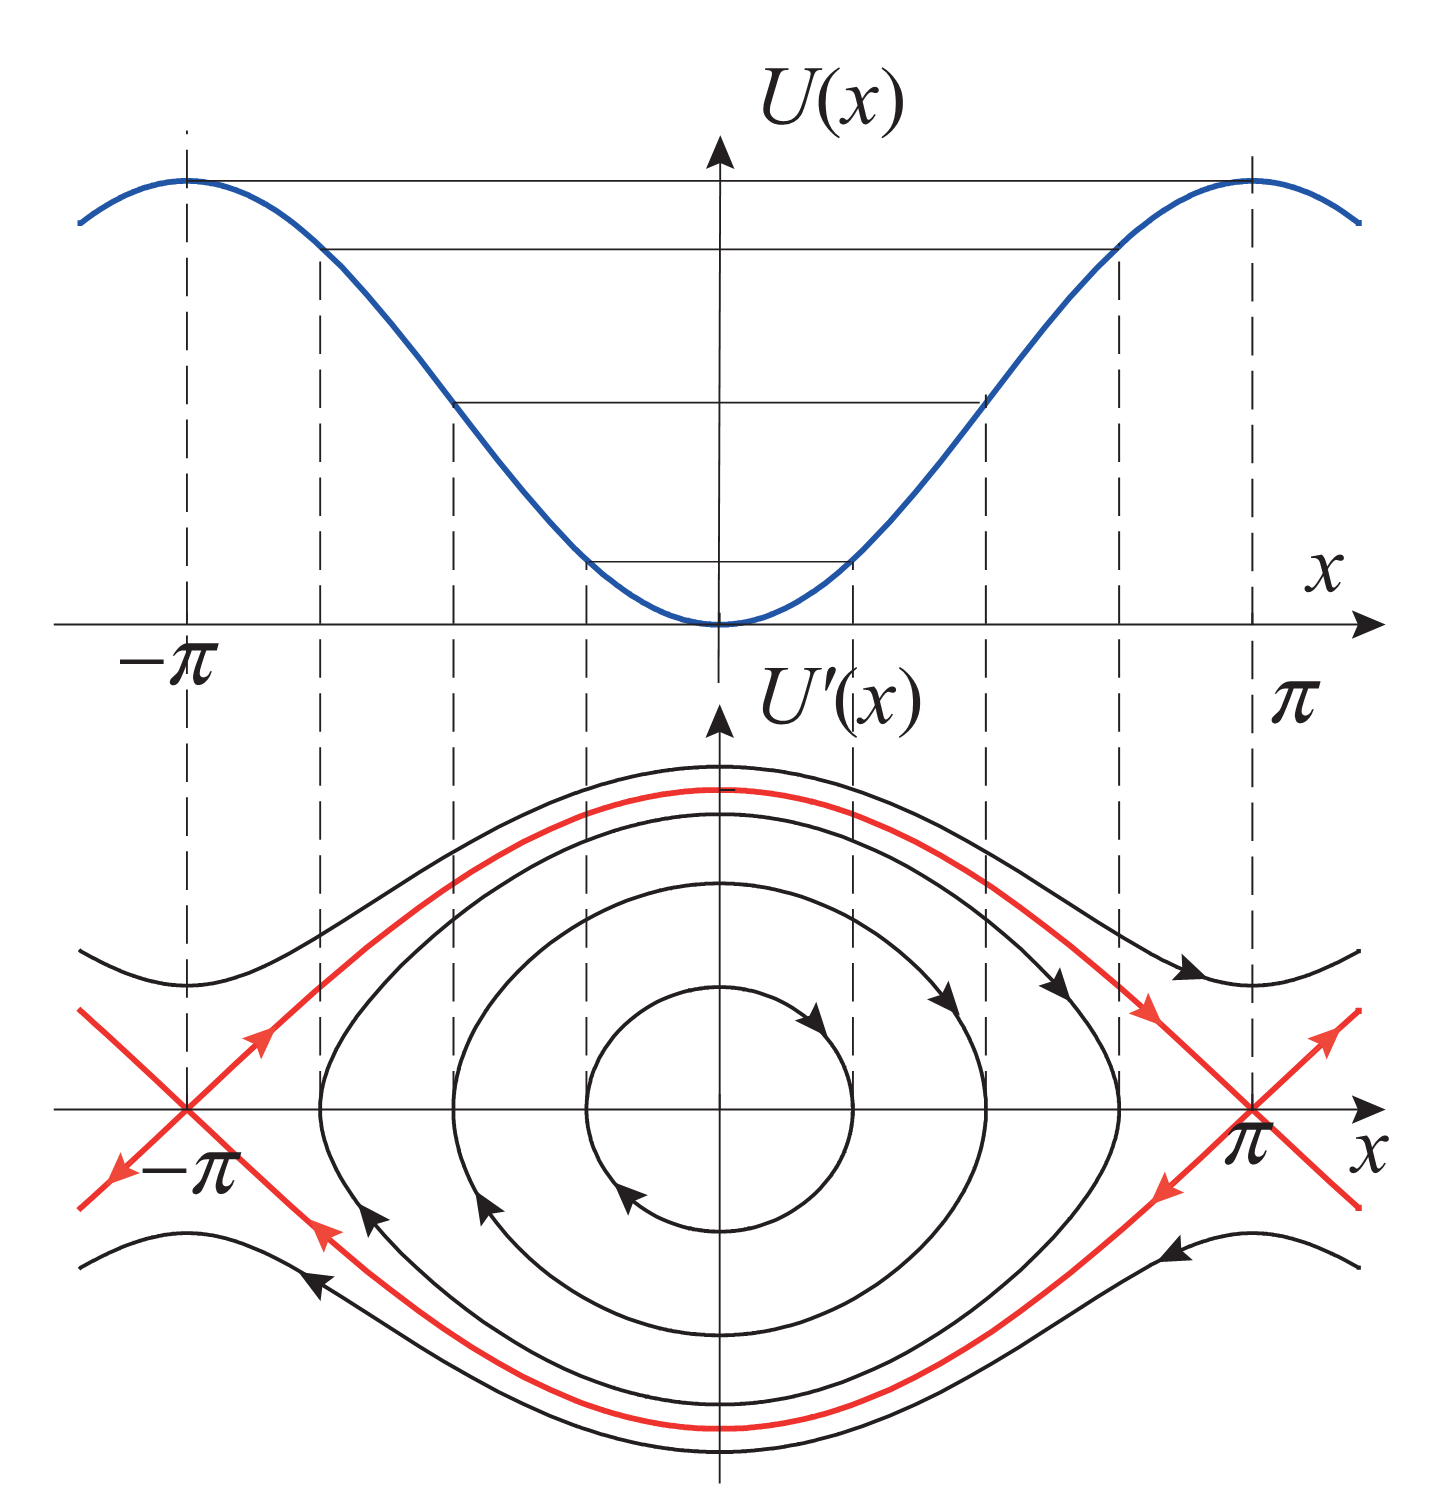
\includegraphics{graphs/pendul-fase_1.png}
	\end{center}

\end{ejer}
